% 11-45 pages (27 on average)
% aim for 2-5 pages for each major section
\chapter{Background}\label{chapter:background}

% ---both are used mainly in \cref{chapter:randomlps}

This chapter provides a brief overview of the concepts and topics pertinent to
the rest of the thesis. We start in \cref{sec:proplogic} with a description of
propositional logic and the kinds of computational problems that use a
logic-based input format or are closely tied to logic in some other way. Then,
\cref{sec:declarative} introduces two declarative programming paradigms that can
be used to describe various computational problems: logic programming and
constraint programming. Next, \cref{sec:representations} covers various ways to
represent probability distributions. We divide these representations into those
based on graphs (i.e., probabilistic graphical models) and those based on text
(i.e., probabilistic programming languages). Likewise, \cref{sec:kc} covers
various representations of Boolean and pseudo-Boolean functions. These
representations (and algorithms that compile into them) are crucial in many WMC
and probabilistic inference algorithms. We end the chapter with
\cref{sec:applications}, which provides an overview of the applications of WMC
and its impact on areas such as bioinformatics, natural language processing, and
robotics.

\section{Propositional Logic}\label{sec:proplogic}

In this section, we briefly introduce the fundamentals of propositional logic
and describe some logic-based computational problems. We refer the reader to the
book by \citet{DBLP:books/daglib/0029942} for a more detailed introduction to
logic and its role in computer science.

An \emph{atomic proposition} (also known as an \emph{atom} or a
\emph{Boolean/logical/propositional variable}) is a variable with two possible
(truth) values: \true{} and \false{}. We usually refer to atoms as
\emph{variables}. A \emph{formula} is any well-formed expression that connects
variables using the following Boolean/logical operators (and parentheses):
negation ($\neg$), disjunction ($\lor$), conjunction ($\land$), (material)
implication ($\Rightarrow$), and equivalence (i.e., material biconditional,
$\Leftrightarrow$). The last two operators are often defined as
$a \Rightarrow b \equiv \neg a \lor b$ and
$a \Leftrightarrow b \equiv (a \Rightarrow b) \land (b \Rightarrow a)$. A
\emph{literal} is either a variable or its negation, respectively called
\emph{positive} and \emph{negative} literal. A \emph{clause} is a disjunction of
literals.\footnote{The word \emph{clause} is defined differently in
  \cref{sec:lp,chapter:randomlps,chapter:wfomc}.} A formula is in
\emph{conjunctive normal form} (CNF) if it is a conjunction of clauses, and it
is in $k$-CNF if every clause has exactly $k$ literals. Many other normal forms
and ways to represent propositional formulas are covered in \cref{sec:kc}.

An \emph{interpretation} (also known as a \emph{variable assignment}) of a
formula $\phi$ is a map from the variables of $\phi$ to the set
$\{\, \true{}, \false{} \,\}$. A \emph{model} is an interpretation under which
$\phi$ evaluates to \true{}. A formula is
\begin{description}
\item[satisfiable] if it has at least one model,
\item[unsatisfiable] (i.e., a \emph{contradiction}) if it has no models, and a
\item[tautology] (i.e., \emph{valid}) if all interpretations are models.
\end{description}
We denote tautologies and contradictions as $\top$ and $\bot$, respectively, and
often use them interchangeably with the truth values \true{} and \false{}. Two
formulas $\phi$ and $\psi$ over the same set of variables are \emph{equivalent}
(denoted $\phi \equiv \psi$) if they have equal sets of models.

Throughout the thesis, we use set-theoretic notation for many concepts in logic
such as clauses and formulas in CNF (e.g., we write $c \in \phi$ to mean that
clause $c$ is one of the clauses of formula $\phi$). However, this does not
automatically mean that no duplicates are allowed---whether or not that is the
case is clarified on a case-by-case basis.

\begin{example}\label{example:logic}
  Formula $\phi \coloneqq (\neg a \lor b) \land a$ has two variables $a$ and
  $b$, is in CNF, and contains two clauses. The first clause $\neg a \lor b$ has
  a negative literal $\neg a$ and a positive literal $b$. Since $\phi$ has two
  variables, it also has four interpretations. Interpretation
  $\{\, a \mapsto \true{}, b \mapsto \true{} \,\}$ is a model, so $\phi$ is
  satisfiable. An equivalent set-theoretic representation of $\phi$ is
  $\{\, \{\, \neg a, b \,\}, \{\, a \,\} \,\}$.
\end{example}

\emph{Primal treewidth} is a parameter we use in \cref{chapter:comparison} to
quantify the structural hardness of a formula. The primal treewidth of a CNF
formula $\phi$ is the treewidth of the primal graph of $\phi$. The \emph{primal
  graph} of a CNF formula is a graph that has a node for every variable, and
there is an edge between two variables if they coappear in some clause. The
\emph{treewidth} of a graph $G$ measures how similar $G$ is to a tree and is
stated in \cref{def:treewidth}. Primal treewidth (and treewidth more generally)
is a parameter frequently used to describe the parameterised complexity of
algorithms
\citep{DBLP:conf/ijcai/BliemMMW17,DBLP:series/txcs/DowneyF13,DBLP:conf/lics/FichteHP20}.
For a graph $G$, let $\mathcal{V}(G)$ denote the set of nodes of $G$ and
$\mathcal{E}(G)$ denote the set of edges of $G$.

\begin{definition}[\cite{DBLP:journals/jct/RobertsonS84}]\label{def:treewidth}
  A \emph{tree decomposition} of a graph $G$ is a pair $(T, \chi)$, where $T$ is
  a tree and $\chi\colon \mathcal{V}(T) \to 2^{\mathcal{V}(G)}$ is a labelling
  function, with the following properties:
  \begin{itemize}
    \item $\bigcup_{t \in \mathcal{V}(T)} \chi(t) = \mathcal{V}(G)$;
    \item for every edge $e \in \mathcal{E}(G)$, there is $t \in \mathcal{V}(T)$
          such that $e$ has both endpoints in $\chi(t)$;
    \item for all $t, t', t'' \in \mathcal{V}(T)$, if $t'$ is on the path
          between $t$ and $t''$, then
          $\chi(t) \cap \chi(t'') \subseteq \chi(t')$.
  \end{itemize}
  The \emph{width} of tree decomposition $(T, \chi)$ is
  $\max_{t \in \mathcal{V}(T)} |\chi(t)| - 1$. The \emph{treewidth} of graph $G$
  is the smallest $w$ such that $G$ has a tree decomposition of width $w$.
\end{definition}

\begin{figure}
  \centering
  \begin{subfigure}[b]{0.29\textwidth}
    \centering
    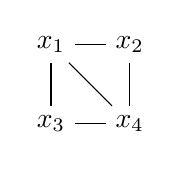
\begin{tikzpicture}
      \node (one) at (0, 1) {$x_1$};
      \node (two) at (1, 1) {$x_2$};
      \node (three) at (0, 0) {$x_3$};
      \node (four) at (1, 0) {$x_4$};
      \draw (one) -- (two);
      \draw (one) -- (three);
      \draw (one) -- (four);
      \draw (two) -- (four);
      \draw (three) -- (four);
    \end{tikzpicture}
  \caption{the primal graph of $\phi$}\label{fig:primal}
  \end{subfigure}
  \begin{subfigure}[b]{0.69\textwidth}
    \centering
    \begin{tikzpicture}[every text node part/.style={align=center}]
      \node[circle,draw] (one) {$x_1$ $x_2$\\$x_4$};
      \node[circle,draw,right=of one] (two) {$x_1$ $x_3$\\$x_4$};
      \draw (one) -- (two);
    \end{tikzpicture}
    \caption{a minimum-width tree decomposition of the primal
      graph}\label{fig:decomposition}
  \end{subfigure}
  \caption{Two graphs associated with formula $\phi$ from
    \cref{example:treewidth}}\label{fig:decompositions}
\end{figure}

\begin{example}\label{example:treewidth}
  Let $\phi$ be the formula
  $(x_{4} \lor \neg x_{3} \lor x_{1}) \land (\neg x_{2} \lor x_{4}) \land (\neg x_{1} \lor x_{2} \lor x_{4})$.
  The primal graph of $\phi$ is pictured in \cref{fig:primal}; it is one edge
  away from being a complete graph since only $x_{2}$ and $x_{3}$ do not appear
  in a clause together. \Cref{fig:decomposition} shows a tree decomposition of
  the primal graph of width 2. Since the graph in \cref{fig:primal} does not
  have a tree decomposition of width 1, the treewidth of the primal graph is 2,
  and thus the primal treewidth of $\phi$ is also 2.
\end{example}

\subsection{Logic-Based Computational Problems}\label{sec:logicproblems}

% applications of MC:
% * automatically synthesizing search algorithms \citep{DBLP:journals/corr/abs-2009-10877}
% * model counting: assessing the quality of an explanation of a machine learning model \citep{DBLP:conf/sat/NarodytskaSMIM19}
% * model counting: analysing software for vulnerabilities \citep{DBLP:conf/sp/ZhouQRZ18}

We begin with a description of SAT and some of its extensions. Given a
propositional formula\footnote{Unless stated otherwise, formulas for SAT and
  other similar problems are assumed to be in CNF.}, SAT asks whether the
formula is satisfiable. SAT (also known as \emph{propositional/Boolean
  satisfiability}) is the first problem shown to be \NP-complete
\citep{DBLP:conf/stoc/Cook71,levin1973universal}. Motivated by many real-life
problems that were found to be reducible to SAT, research in SAT solving
produced algorithms that can efficiently tackle large instances despite the
exponential worst-case time complexity \citep{DBLP:series/faia/2009-185}.

Instead of satisfying all clauses, one can attempt to find an interpretation
that satisfies the maximum number of clauses---this problem is called MaxSAT
\citep{bacchus2021maximum,DBLP:series/faia/LiM09}. It is an \NP-hard
optimisation problem that (in its most general form) attaches a (potentially
infinite) cost for failing to satisfy each clause and seeks to minimise total
cost.

\mc{}, or \emph{(propositional) model counting}, asks to count the number of
models of a formula \citep{DBLP:series/faia/GomesSS09}. \mc{} is the canonical
\#\P-complete problem with many applications in areas such as planning and
probabilistic reasoning. $\#\exists\textrm{SAT}$, or \emph{projected model
  counting}, selects a subset of variables called \emph{priority variables}
\citep{DBLP:conf/sat/AzizCMS15}. The task is then to count the number of
assignments of values to priority variables that can be extended to models. The
extension of \mc{} most relevant to our work is called \emph{weighted model
  counting} (WMC). Given a propositional formula $\phi$ and a \emph{weight
  function} $w$ from the literals of $\phi$ to non-negative real numbers, WMC
asks to compute
\[
\WMC(\phi) = \sum_{\omega \models \phi} \prod_{\omega \models l} w(l),
\]
where the summation is over all models $\omega$ of $\phi$, and the product is
over all literals of $\omega$ \citep{DBLP:journals/ai/ChaviraD08}. Lastly, both
\mc{} and WMC have been extended to first-order logic
\citep{DBLP:conf/ijcai/BroeckTMDR11}---this is the topic of
\cref{chapter:wfomc}.

\begin{example}\label{example:wmc1}
  The model count of the formula in \cref{example:logic} is equal to one. With a
  weight function
  $w \coloneqq \{\, a \mapsto 0.7, \neg a \mapsto 0.2, b \mapsto 0.8, \neg b \mapsto 0.7 \,\}$,
  the WMC of the same formula is $0.7 \times 0.8 = 0.56$.
\end{example}

\begin{example}
  With the same weight function $w$ as in \cref{example:wmc1}, the WMC of
  formula $a \lor b$ is
  $w(a)w(b) + w(a)w(\neg b) + w(\neg a)w(b) = 0.7 \times 0.8 + 0.7 \times 0.7 + 0.2 \times 0.8 = 1.21$,
  and the model count of this formula is 3.
\end{example}

WMC has been extended in many ways to support, e.g., continuous variables
\citep{DBLP:conf/ijcai/BellePB15}, infinite domains
\citep{DBLP:conf/aaai/Belle17}, and function symbols
\citep{DBLP:conf/uai/Belle17}. In particular, the extension to first-order
logic, known as \emph{(symmetric) weighted first-order model counting} (WFOMC)
\citep{DBLP:journals/cacm/GogateD16,DBLP:conf/ijcai/BroeckTMDR11} is the focus
of \cref{chapter:wfomc}. There is also recent work providing support for both
continuous variables and first-order logic \citep{DBLP:conf/uai/FeldsteinB21}.
Finally, replacing real numbers with addition and multiplication with an
arbitrary commutative semiring allows WMC to subsume a variety of other problems
such as most probable explanation, shortest path, and gradient computation
\citep{DBLP:journals/ijar/BelleR20,DBLP:journals/japll/KimmigBR17}.

There are a number of other computational problems that similarly use logical or
algebraic constructs to encode problems from various domains. First, a
propositional formula with prepended quantifiers for all of its variables is
known as a \emph{quantified Boolean formula} \citep{DBLP:series/faia/BuningB09}.
One can then ask whether the formula is true or false. \emph{Satisfiability
  module theories} considers SAT in the context of a background theory
\citep{DBLP:series/faia/BarrettSST09}. These theories can describe the
properties of integer arithmetic, sets, trees, strings, and many commonly-used
abstract data structures. \emph{Pseudo-Boolean} solvers consider decision and
optimisation problems that can be expressed as linear inequalities over Boolean
variables \citep{DBLP:series/faia/RousselM09}. \emph{Integer (linear)
  programming} instances encode integer optimisation problems under inequality
constraints of a certain linear-algebraic form \citep{wolsey2020integer}.
Finally, \emph{constraint programming} is a powerful paradigm for solving
combinatorial search and optimisation problems with a much more expressive
syntax \citep{DBLP:reference/fai/2}---we discuss constraint programming in more
detail in \cref{sec:cp}.

\section{Declarative Programming}\label{sec:declarative}

In contrast to imperative programming, in a declarative programming language,
one describes \emph{what} is to be computed but not \emph{how}. Here we describe
two declarative programming paradigms pertinent to our work: logic programming
and constraint programming.

\subsection{Logic Programming}\label{sec:lp}

In this subsection, we give a brief introduction to logic programming.
Specifically, we focus on Prolog---the most popular logic programming language
yet. We do not, however, attempt to cover all (or even most) of the capabilities
of Prolog but rather focus on the main concepts and ideas relevant to our work
in \cref{chapter:randomlps}. Note that different descriptions of logic
programming often use different (and mutually inconsistent) terminologies. Here
we prioritise names and definitions that are sufficiently general for our needs
and reasonably consistent with the terminology used in logic. For more details
on logic programming and Prolog, we refer the reader to some of the numerous
books on the subject
\citep{DBLP:books/daglib/0041598,DBLP:books/daglib/0067951}.

A \emph{logic program} is a finite sequence\footnote{Although it is common to
  define logic programs as sets, the order is important for efficiency and can
  be the difference between finite and infinite running time.} of clauses. A
\emph{clause} consists of a head and a body. If a clause has an empty body, it
is a \emph{fact}; otherwise it is a \emph{rule}. The Prolog syntax for a fact
and a rule is \verb+h.+ and \verb+h :- b.+, respectively, where \texttt{h} is
the head and \texttt{b} is the body, although we often write
$\texttt{h} \gets \texttt{b}$ instead.

The \emph{head} of a clause is an atom. An \emph{atom} (i.e., atomic formula)
has the form $p(t_1, \dots, t_n)$, where $p$ is a \emph{predicate (symbol)}, and
${(t_i)}_{i=1}^n$ are terms. Here, $n \in \mathbb{N}_0$ is the \emph{arity} of
$P$. When the arity is equal to zero, the atom is also known as a
\emph{propositional variable}. Some built-in predicates such as equality can be
written in infix notation and without parentheses, i.e., as $a = b$ instead of
$=(a, b)$. A \emph{term} is either a \emph{(logical) variable} (i.e., a string
that begins with a capital letter) or a \emph{constant} (i.e., any other
string). If an atom contains only constants, it is a \emph{ground} atom.

The \emph{body} of a clause is a formula.\footnote{In the literature, it is
  common to define clause bodies as conjunctions, but here we present a more
  general definition, given that such a generalisation is widely supported by
  the relevant software.} A \emph{formula} is any well-formed expression that
connects atoms using conjunction, disjunction, and negation (as well as
parentheses). Prolog syntax for these operators is different from the standard
notation used in logic: we write `\verb+,+' instead of $\land$, `\verb+;+'
instead of $\lor$, and `\verb#\+#' instead of $\neg$. Just like with the syntax
for clauses, in most cases we continue to use logic-based syntax for
convenience.

Finally, a \emph{query} is a formula to be evaluated. If the query has no
variables, the evaluation returns either \true{} or \false{}. Otherwise, the
logic programming engine tries to replace the variables of the query with
constants such that the resulting formula is a logical consequence of the
program. If successful, an example of such a mapping is returned; if not, the
engine returns \false{}.

\begin{example}
  Consider the following logic program.
\begin{verbatim}
parent(sky, will).
parent(will, zoe).
ancestor(X, Z) :- parent(X, Z); (parent(X, Y), ancestor(Y, Z)).
\end{verbatim}
  In our alternative logic-based notation, the last clause could also be written
  as
  \[
    \texttt{ancestor(X, Z)} \gets \texttt{parent(X, Z)} \lor (\texttt{parent(X, Y)} \land \texttt{ancestor(Y, Z)}).
  \]

  This program has three clauses. The first two clauses are facts, whereas the
  last clause is a rule. The program uses two predicates (\texttt{parent} and
  \texttt{ancestor}), three constants (\texttt{sky}, \texttt{will}, and
  \texttt{zoe}), and the last clauses uses three variables (\texttt{X},
  \texttt{Y}, and \texttt{Z}). Both predicates are of arity 2.

  Clause-by-clause, this program can be interpreted as:
  \begin{itemize}
    \item Sky is a parent of Will.
    \item Will is a parent of Zoe.
    \item \texttt{X} is an ancestor of \texttt{Z} if \texttt{X} is a parent of
          \texttt{Z} or there is a \texttt{Y} such that \texttt{X} is a parent
          of \texttt{Y}, and \texttt{Y} is an ancestor of \texttt{Z}.
  \end{itemize}

  The query \texttt{ancestor(sky, zoe)} returns \true{} since Sky is a parent of
  a parent of Zoe, and thus an ancestor. The query \texttt{ancestor(X, sky)}
  returns \false{} because we know nothing about the ancestors of Sky. Lastly,
  the query \texttt{ancestor(sky, X)} could return either
  $\{\, \texttt{X} \mapsto \texttt{will} \,\}$ or
  $\{\, \texttt{X} \mapsto \texttt{zoe} \,\}$ as both Will and Zoe have Sky as
  an ancestor.
\end{example}

% could also describe stratification in more detail (either here or in Chapter 3)

%% \paragraph*{Things to mention.}
%% \begin{itemize}
%% \item we're not defining literals here
%% \item the generalisation of clauses affects the definitions of stratification and dependency graph as well
%% \item Stratification
%%   \begin{itemize}
%%   \item \emph{Stratification} is a condition necessary for probabilistic logic programs
%%     \citep{DBLP:conf/padl/MantadelisR17} and often enforced on logic programs
%%     \citep{DBLP:journals/tcs/Bidoit91} that helps to ensure a unique answer to every
%%     query. This is achieved by restricting the use of negation so that any program
%%     $\mathscr{P}$ can be partitioned into a sequence of programs $\mathscr{P} =
%%     \bigsqcup_{i=1}^n \mathscr{P}_i$ such that, for all $i$, the negative literals
%%     in $\mathscr{P}_i$ can only refer to predicates defined in $\mathscr{P}_j$ for
%%     $j \le i$ \citep{DBLP:journals/tcs/Bidoit91}.
%%   \item include the formal definition from the original paper \citep{DBLP:books/mk/minker88/AptBW88}
%%   \item also include a good example
%%   \item consider including the definition of a (predicate) dependency graph and the lemma that follows. I think the original definition is slightly different: it allows edges to be positive and negative at the same time.
%%   \item (the original paper) shown that stratified programs are always consistent (i.e., avoid paradoxical situations such as $p \gets \neg p$) \citep{DBLP:books/mk/minker88/AptBW88}
%%   \item only a sufficient condition for consistency
%%   \end{itemize}
%% \end{itemize}

\subsection{Constraint Programming}\label{sec:cp}

Constraint models are successfully used to tackle search problems in many
domains such as bioinformatics, configuration, networks, planning, scheduling,
and vehicle routing \citep{DBLP:reference/fai/2}. Here we briefly describe what
a constraint satisfaction problem (CSP) is, how an algorithm might attempt to
solve it, and how one can help the algorithm search efficiently.

\begin{definition}
  A \emph{CSP} is a triple $(X, D, C)$, where
  \begin{itemize}
    \item $X = {(x_i)}_{i=1}^n$ is an $n$-tuple of variables,
    \item $D = {(D_i)}_{i=1}^n$ is an $n$-tuple of (typically, finite) domains
          such that $x_i \in D_i$,
    \item and $C$ is a set of constraints.
  \end{itemize}
  A \emph{constraint} is a pair $(S, R)$, where $S \subseteq X$ is the
  \emph{scope} of the constraint, and $R \subseteq \prod_{x_i \in S} D_i$ is a
  relation specifying allowed combinations of values. Constraints can be
  specified either \emph{intensionally} (i.e., by describing a formula that must
  be satisfied) or \emph{extensionally} (i.e., by listing all tuples). A
  \emph{solution} to the CSP is an $n$-tuple ${(a_i)}_{i=1}^n$ such that
  $a_i \in D_i$ and the relevant $a_i$'s are in the relations of all the
  constraints in $C$.
\end{definition}

\begin{example}[$n$ queens]\label{example:n_queens}
  Imagine an $n \times n$ chess board. How can one place $n$ queens on the board
  so that no two queens threaten each other (i.e., are not on the same column,
  row, or diagonal)? This is the famous \emph{$n$ queens problem}---a common
  example in the constraint programming literature. The solution we describe
  here is adapted from a constraint modelling tutorial \citep{minizinc}.

  First, note that each column (i.e, \emph{file}) must have exactly one queen.
  Let ${(q_i)}_{i=1}^n$ be variables with domains
  $q_i \in \{\, 1, \dots, n \,\}$, where we use $q_i = j$ to denote that the
  $i$\textsuperscript{th} column queen is on row (i.e., \emph{rank}) $j$. Then
  the entire problem can be described by the following three constraints.

  \begin{constraint}\label{exampleconstraint:1}
    $\alldifferent({\{\, q_i \,\}}_{i=1}^n)$
  \end{constraint}

  \begin{constraint}\label{exampleconstraint:2}
    $\alldifferent(\{\, q_i + i \mid i = 1, \dots, n \,\})$
  \end{constraint}

  \begin{constraint}\label{exampleconstraint:3}
    $\alldifferent(\{\, q_i - i \mid i = 1, \dots, n \,\})$
  \end{constraint}

  Here, $\alldifferent$ is a constraint on a set of variables (or `derivatives'
  of variables) that constrains them to be all different.
  \Cref{exampleconstraint:1} requires all queens to occupy different rows, and
  \cref{exampleconstraint:2,exampleconstraint:3} do the same for both diagonals.

  Note that, given one solution to the $n$-queens problem, we can easily find
  seven others just by rotating and flipping the board in every possible way
  (i.e., the symmetry group of a square has order 8). Thus, there is no reason
  for the constraint solver to find all eight symmetrical solutions
  independently. Avoiding this kind of excessive effort is the goal of
  \emph{symmetry breaking} constraints.

  While some symmetry breaking constraints can be expressed using variables
  ${(q_i)}_{i=1}^n$, others could benefit from a different representation.
  Specifically, let $\mathbf{B} = (b_{ij})$ be an $n \times n$ matrix, where
  each $b_{ij} \in \{\, \true{}, \false{} \,\}$ indicates whether the
  $(i,j)$\textsuperscript{th} square contains a queen. Constraints that connect
  different representations of the same problem are called \emph{channelling}
  constraints. In this case, the following constraint is sufficient.

  \begin{constraint}[Channelling]
    For all $i, j = 1, \dots, n$, we have that $b_{ij} \iff (q_i = j)$.
  \end{constraint}

  Finally, the following is an example of a symmetry breaking constraint.

  \begin{constraint}[Symmetry breaking]
    $\mathbf{B}$ is lexicographically smaller than or equal to $\mathbf{B}^\top$
    (i.e., the transpose of $\mathbf{B}$).
  \end{constraint}
\end{example}

Perhaps the most canonical way of solving a CSP is by \emph{backtracking
  search}. At each step, the algorithm selects a variable $x_i$, a value
$v \in D_i$, sets
\begin{equation} \label{eq:decision}
  x_i \coloneqq v,
\end{equation}
and continues this process until either all constraints are satisfied or some
constraint can no longer be satisfied.

Sometimes making a \emph{decision} (i.e., setting a variable to be equal to a
value as in \cref{eq:decision}) leads to other variable-value combinations
becoming evidently impossible. For example, after placing a queen on a1 (i.e.,
setting $q_1 \coloneqq 1$), \cref{exampleconstraint:1} tells us that no other
queen can be placed on the first row (i.e., $q_i \ne 1$ for all
$i = 2, \dots, n$). Purging such impossible values from domains is the job of
\emph{(constraint) propagation} (or \emph{inference}) algorithms. These
algorithms are designed separately for each type of constraint and vary in their
complexity and efficacy (i.e., how many values they are able to remove).

Another issue that needs to be addressed on a per-constraint basis is: how do we
know when a constraint is satisfied? Indeed, if all constraints are already
satisfied, then it must be the case that setting all remaining variables to
\emph{any} values produces a valid solution. This problem is known as
\emph{entailment}. Entailment algorithms take a CSP with a (potentially partial)
variable-value assignment and return one out of three possible values:
\begin{description}
\item[true] if the constraint is already satisfied,
\item[false] if it is impossible to satisfy the constraint,
\item[maybe/undefined] if neither of the above is seemingly the case.
\end{description}

Backtracking search has important choices to make: which variable should be
given a value first? Which value from a domain is most likely to lead to a
solution? These questions are answered by \emph{variable} and \emph{value
  ordering heuristics}, respectively. For example, we can choose a variable with
the smallest number of values remaining in its domain---this is known as the
\emph{dom}, \emph{smallest domain first}, or \emph{first fail} heuristic. Value
ordering heuristics typically consider what the sizes of all domains would be
given each instantiation of the selected variable and choose the value that
minimises either their sum or their product \citep{DBLP:reference/fai/Beek06}.
Both kinds of heuristics can also be random, e.g., a variable or a value can be
sampled from a uniform distribution. Random heuristics are typically combined
with a \emph{restart strategy} that decides how long the search should continue
before assuming that a mistake must have been made and restarting the search
\citep{DBLP:reference/fai/Beek06}.

\section{Representations of Probability
  Distributions}\label{sec:representations}

In what follows, we assume that the reader is familiar with the basic ideas of
probability theory. For reference, one might wish to consult a book by, e.g.,
\citet{loeve} or \citet{stroock2010probability} for a comprehensive treatment of
probability theory and its measure-theoretic foundations. Unless specified
otherwise, by \emph{probability distribution} we mean a \emph{discrete}
probability distribution. Moreover, we are typically only interested in
probability distributions with \emph{finite support}. With these restrictions,
one could define a probability distribution by listing all combinations of
values and assigning a probability to each. However, in most realistic
scenarios, the same information could be described more succinctly by taking
advantage of concepts such as random variable \emph{independence},
\emph{conditional independence}, and \emph{exchangeability}. In this section, we
describe some representations of probability distributions and their semantics.
\Cref{sec:pgms} is about representations based on graphs, whereas
\cref{sec:probprogramming} covers probabilistic programming languages. These
representations also differ in their ability to reason about sets of random
variables. \emph{Propositional} models treat each random variable as a unique
individual. In contrast, \emph{relational} models work over sets of individuals
and relations among them. See the book by
\citet{DBLP:series/synthesis/2016Raedt} for more detail.

\subsection{Representations Based on Graphical Models}\label{sec:pgms}

Perhaps the best-known representations of probability distributions are
\emph{probabilistic graphical models} (PGMs), i.e., probabilistic models that
use a graph-based representation to compactly encode a probability distribution.
These graphs can be either directed (as in the case of Bayesian networks) or
undirected (as in the case of Markov networks). This section provides a brief
overview of these two networks although there are also other PGMs such as factor
graphs \citep{DBLP:journals/spm/Loeliger04,DBLP:series/synthesis/2016Raedt} as
well as graphical models that capture concepts other than probabilities, e.g.,
constraint networks, cost networks, and influence diagrams
\citep{DBLP:series/synthesis/2019Dechter}. For more information on PGMs, see
some of the many books on the subject
\citep{DBLP:series/synthesis/2019Dechter,DBLP:books/daglib/0023091,DBLP:books/daglib/0066829}.

\begin{example}[A classic example]\label{example:bn}
  Suppose you have a burglar alarm in your home. The alarm is likely (but not
  guaranteed) to be activated when a burglar enters, but it might also be
  activated by a larger earthquake or even for no apparent reason. (There might
  even be an earthquake at the time of a burglary!) Furthermore, suppose you
  have two neighbours: John and Mary. Independently, either of them might call
  you if they hear your alarm ringing or for some other reason. Let the
  following (binary) random variables denote the relevant events:
  \begin{description}
  \item[$B$]--- a burglar entering your home,
  \item[$E$]--- an earthquake happening near your home,
  \item[$A$]--- your burglar alarm activating,
  \item[$J$]--- John calling you,
  \item[$M$]--- Mary calling you.
  \end{description}
\end{example}

\begin{figure}[t]
  \centering
  \begin{subfigure}{0.49\textwidth}
    \centering
    \begin{tikzpicture}[node distance=1.5cm]
      \node[draw,circle] (alarm) {A};
      \node[draw,circle,above left of=alarm] (burglary) {$B$};
      \node[draw,circle,above right of=alarm] (earthquake) {$E$};
      \node[draw,circle,below left of=alarm] (johnCalls) {$J$};
      \node[draw,circle,below right of=alarm] (maryCalls) {$M$};
      \draw[-Latex] (burglary) -- (alarm);
      \draw[-Latex] (earthquake) -- (alarm);
      \draw[-Latex] (alarm) -- (johnCalls);
      \draw[-Latex] (alarm) -- (maryCalls);
    \end{tikzpicture}
    \caption{a Bayesian network}\label{fig:bn}
  \end{subfigure}
  \begin{subfigure}{0.49\textwidth}
    \centering
    \begin{tikzpicture}[node distance=1.5cm]
      \node[draw,circle] (alarm) {A};
      \node[draw,circle,above left of=alarm] (burglary) {$B$};
      \node[draw,circle,above right of=alarm] (earthquake) {$E$};
      \node[draw,circle,below left of=alarm] (johnCalls) {$J$};
      \node[draw,circle,below right of=alarm] (maryCalls) {$M$};
      \draw[color=color1,ultra thick] (burglary) -- (earthquake);
      \draw[color=color1,ultra thick] (burglary) -- (alarm);
      \draw[color=color1,ultra thick] (earthquake) -- (alarm);
      \draw[color=color2,ultra thick] (alarm) -- (johnCalls);
      \draw[color=color3,ultra thick] (alarm) -- (maryCalls);
    \end{tikzpicture}
    \caption{a Markov network}\label{fig:mn}
  \end{subfigure}
  \caption{Two PGMs that describe the independence structure of \cref{example:bn}.}
\end{figure}

\begin{table}[t]
  \centering
  \begin{tabular}[t]{lllr}
    \toprule
    $b$ & $e$ & $a$ & $\Pr(A = a \mid B = b, E = e)$ \\
    \midrule
    \rowcolor{gray!25}\multicolumn{2}{c}{} & \false{} & 0.999 \\
    \rowcolor{gray!25}\multicolumn{2}{c}{\multirow{-2}{*}{\false{}}} & \true{} & 0.001 \\
    & & \false{} & 0.71 \\
    \multirow{-2}{*}{\false{}} & \multirow{-2}{*}{\true{}} & \true{} & 0.29 \\
    \rowcolor{gray!25}& & \false{} & 0.06 \\
    \rowcolor{gray!25}\multirow{-2}{*}{\true{}} & \multirow{-2}{*}{\false{}} & \true{} & 0.94 \\
    \multicolumn{2}{c}{} & \false{} & 0.05 \\
    \multicolumn{2}{c}{\multirow{-2}{*}{\true{}}} & \true{} & 0.95 \\
    \bottomrule
  \end{tabular}
  \caption{An example CPT for $\Pr(A \mid B, E)$ from
    \cref{example:bn}.}\label{table:examplecpt}
\end{table}

The graph of a \emph{Bayesian network} for this example scenario is in
\cref{fig:bn}. This directed acyclic graph (DAG) tells us that the joint
probability distribution can be factored as
\begin{equation} \label{eq:factorisation}
  \Pr(B, E, A, J, M) = \Pr(B) \times \Pr(E) \times \Pr(A \mid B, E) \times \Pr(J \mid A) \times \Pr(M \mid A),
\end{equation}
i.e., the probability of each random variable is conditioned on its parents in
the graph. The factors in \cref{eq:factorisation} can be described using
\emph{conditional probability tables} (CPTs). CPTs assign a probability to each
combination of values that the random variable and its parents can take---see
\cref{table:examplecpt} for an example.

Alternatively, the same probability distribution can be represented as an
undirected PGM known as a \emph{Markov network} (or \emph{Markov random field}).
The graph of such a network for \cref{example:bn} is in \cref{fig:mn}. Here,
instead of CPTs, \emph{potentials} are the building blocks out of which a
probability distribution is constructed. A potential is a function from (some
subset of) random variables to non-negative real numbers. Potentials are
typically defined on the maximal cliques of the network. The edge sets of the
three maximal cliques in \cref{fig:mn} are highlighted in different colours.
Thus, the full probability distribution can be factored as
\[
\Pr(B, E, A, J, M) = \frac{1}{Z} \times \psi_1(B, E, A) \times \psi_2(A, J) \times \psi_3(A, M),
\]
where $\psi_1$, $\psi_2$, and $\psi_3$ are potentials, and $Z$ is a
normalisation constant known as the \emph{partition function}.

What if we wanted to generalise \cref{example:bn} to support any number of
neighbours, all of whom behave identically (i.e., have the same probabilities of
calling in all circumstances)? Both Bayesian and Markov networks have been
extended for such scenarios: \emph{relational Bayesian networks}
\citep{DBLP:conf/uai/Jaeger97} can compactly describe a probability distribution
over a relational structure, and \emph{Markov logic networks} (also known as
\emph{Markov logic}) \citep{DBLP:journals/ml/RichardsonD06} extend Markov
networks with support for first-order logic. The field of learning such
representations from data is known as \emph{statistical relational learning}
\citep{DBLP:series/synthesis/2016Raedt}. The next section describes relational
representations that are based on programming languages instead of graphical
models.

\subsection{Probabilistic Programming}\label{sec:probprogramming}

% BLOG \citep{DBLP:conf/ijcai/MilchMRSOK05}, NP-BLOG \citep{DBLP:conf/uai/CarbonettoKFP05}

Augmenting a programming language with probabilities is another common way to
compactly represent probability distributions. Logic programming languages, in
particular, have been frequently used for this purpose. Examples of
probabilistic logic programming languages include the independent choice logic
\citep{DBLP:journals/ai/Poole97,DBLP:conf/ilp/Poole08}, PRISM
\citep{DBLP:conf/ijcai/SatoK97,DBLP:conf/ilp/SatoK08}, ProbLog
\citep{DBLP:conf/ijcai/RaedtKT07} and CP-logic
\citep{DBLP:journals/tplp/VennekensDB09}. Functional and imperative programming
languages have also seen some use, examples of which include BUGS
\citep{gilks1994language}, IBAL \citep{DBLP:conf/ijcai/Pfeffer01}, Church
\citep{DBLP:conf/uai/GoodmanMRBT08}, and Stan \citep{stan}. More information on
probabilistic logic programming, probabilistic programming more generally, and
statistical relational artificial intelligence can be found in the work of
\citet{DBLP:conf/ilp/2008p}, \citet{DBLP:conf/icse/GordonHNR14}, and
\citet{DBLP:series/synthesis/2016Raedt}, respectively.

\noindent\begin{minipage}{\linewidth}
\begin{lstlisting}[frame=tb,caption=A ProbLog program that computes
  $\protect{\Pr(B \mid J, M)}$ for the scenario described in \cref{example:bn}.,
  label={lst:problog}]
  neighbour(john).
  neighbour(marry).

  0.001 :: burglary.
  0.002 :: earthquake.

  0.95  :: alarm :- burglary, earthquake.
  0.94  :: alarm :- burglary, \+ earthquake.
  0.29  :: alarm :- \+ burglary, earthquake.
  0.001 :: alarm :- \+ burglary, \+ earthquake.

  0.8   :: calls(X) :- alarm, neighbour(X).
  0.1   :: calls(X) :- \+ alarm, neighbour(X).

  evidence(calls(john)).
  evidence(calls(mary)).
  query(burglary).
\end{lstlisting}
\end{minipage}
% \noindent\begin{minipage}{\linewidth}
% \begin{lstlisting}[escapeinside={(*}{*)},frame=tb,caption=A BLOG
%   program that computes $\protect{\Pr(B \mid J, M)}$ for the scenario described
%   in \cref{example:bn}., label={lst:blog}]
%   type Neighbour;
%   distinct Neighbour John, Mary;

%   random Boolean Burglary   (*$\sim$*) BooleanDistrib(0.001);
%   random Boolean Earthquake (*$\sim$*) BooleanDistrib(0.002);

%   random Boolean Alarm (*$\sim$*) case[Burglary, Earthquake] in {
%     [false, false] -> BooleanDistrib(0.001),
%     [false, true]  -> BooleanDistrib(0.29),
%     [true, false]  -> BooleanDistrib(0.94),
%     [true, true]   -> BooleanDistrib(0.95)
%   };

%   random Boolean Calls(Neighbour n) (*$\sim$*)
%     if Alarm then BooleanDistrib(0.8)
%     else BooleanDistrib(0.1);

%   obs Calls(John) = true;
%   obs Calls(Mary) = true;
%   query Burglary;
% \end{lstlisting}
% \end{minipage}

\Cref{lst:problog} contains a probabilistic program that encodes the
information in \cref{example:bn}. In preparation for \cref{chapter:randomlps},
let us examine the syntax and semantics of ProbLog more closely. ProbLog clauses
are exactly like Prolog clauses (see \cref{sec:lp}) but with \verb+p ::+
prepended, for some probability \texttt{p}. Without \verb+::+, the probability
associated with the clause is implicitly equal to 1. ProbLog also has keywords
\texttt{evidence} and \texttt{query} that are used to define one or more
(potentially conditional) probabilities of interest. Reading off the
probabilities from \cref{lst:problog}, we can, e.g., compute the probability
that John calls as
\begin{align*}
  \Pr(j) &= \Pr(b)\Pr(e)\Pr(a \mid b, e)\Pr(j \mid a) \\
  &+ \Pr(b)\Pr(e)\Pr(\neg a \mid b, e)\Pr(j \mid \neg a) \\
  &+ \cdots \\
  &+ \Pr(\neg b)\Pr(\neg e)\Pr(\neg a \mid \neg b, \neg e)\Pr(j \mid \neg a) \\
  &= 0.001 \times 0.002 \times 0.95 \times 0.8 + \cdots \\
  &\approx 0.102.
\end{align*}
More formally, the probability of a query is the sum of the probabilities of the
models of the query (c.f. WMC).

\section{Knowledge Compilation and Representation}\label{sec:kc}
% Probabilistic SDDs \citep{DBLP:conf/kr/KisaBCD14} extend SDDs with probability
% labels on edges.

\emph{Knowledge compilation} is the process of transforming the initial
representation of some data (usually based on propositional logic) to a
representation that allows one to perform various operations and answer queries
of interest in time polynomial in the size of this new representation. Many such
representations have been proposed \citep{DBLP:journals/jair/DarwicheM02}.
Amongst them, those particularly relevant to WMC and probabilistic inference
are:
\begin{itemize}
  \item deterministic decomposable negation normal form (d-DNNF)
        \citep{DBLP:journals/jancl/Darwiche01},
  \item sentential decision diagrams (SDDs) \citep{DBLP:conf/ijcai/Darwiche11},
  \item (ordered) binary decision diagrams (BDDs)
        \citep{DBLP:journals/tc/Bryant86},
  \item and algebraic decision diagrams (ADDs)
        \citep{DBLP:journals/fmsd/BaharFGHMPS97}.
\end{itemize}
The first two items on this list are described in \cref{sec:nnf,sec:sdds},
respectively, and the last two are covered in more detail in \cref{sec:dds}.
While knowledge compilation is a process (which is performed by algorithms),
here our focus is on the representations themselves.

\subsection{NNF and d-DNNF}\label{sec:nnf}

\begin{definition}
  A propositional formula $\phi$ is in \emph{negation normal form} (NNF) if
  \begin{itemize}
    \item the only operators in $\phi$ are $\neg$, $\lor$, and $\land$,
    \item and $\neg$ is only applied to directly to variables.
  \end{itemize}
\end{definition}

\begin{example}
  Formula $\neg(C \Rightarrow (\neg A \land B))$ can be transformed into NNF as
  follows:
  \[
  \neg(C \Rightarrow (\neg A \land B)) \equiv \neg(\neg C \lor (\neg A \land B)) \equiv C \land (A \lor \neg B)
  \]
  using the definition of $\Rightarrow$ and De Morgan's laws.
\end{example}

\begin{definition}
  The d-DNNF adds decomposability and determinism to the NNF\@.
  \emph{Decomposability} requires that, for every conjunction
  $\bigwedge_{i=1}^n \phi_i$, conjuncts $\phi_i$ and $\phi_j$ have no variables
  in common for all $i \ne j$
  \citep{DBLP:conf/ijcai/Darwiche99,DBLP:journals/jacm/Darwiche01}.
  \emph{Determinism} requires that, for every disjunction
  $\bigvee_{i=1}^n \phi_i$, disjuncts $\phi_i$ and $\phi_j$ contradict each
  other (i.e., $\phi_i \land \phi_j \equiv \bot$) for all $i \ne j$
  \citep{DBLP:journals/jancl/Darwiche01}.
\end{definition}

\begin{example}
  Formula $(A \lor \neg B) \land (A \lor C)$ is neither decomposable nor
  deterministic. It is not decomposable because
  $\{\, A, B \,\} \cap \{\, A, C \,\} = \{\, A \,\} \ne \emptyset$. It is not
  deterministic because, e.g., $A \land \neg B \not\equiv \bot$.
\end{example}

\begin{example}\label{example:ddnnf1}
  Formula $C \land (A \lor \neg B)$ is decomposable but not deterministic. It is
  decomposable because $\{\, C \,\} \cap \{\, A, B \,\} = \emptyset$. It is not
  deterministic because $A \land \neg B \not\equiv \bot$.
\end{example}

\begin{example}
  Formula $B \land C \land [\neg B \lor (A \land B)]$ is deterministic but not
  decomposable. It is deterministic because
  $\neg B \land A \land B \equiv \bot$. It is not decomposable because
  $\{\, B \,\} \cap \{\, A, B \,\} = \{\, B \,\} \ne \emptyset$.
\end{example}

\begin{example}\label{example:ddnnf2}
  Formula $C \land [\neg B \lor (A \land B)]$ is decomposable and deterministic.
  It is decomposable because $\{\, C \,\} \cap \{\, A, B \,\} = \emptyset$, and
  $\{\, A \,\} \cap \{\, B \,\} = \emptyset$. It is deterministic because
  $\neg B \land A \land B \equiv \bot$.
\end{example}

\begin{figure}[t]
  \centering
  \begin{subfigure}{0.32\textwidth}
    \centering
    \begin{tikzpicture}[level distance=1cm,edge from
      parent/.style={draw,-Latex}] % C \land [\neg B \lor (A \land B)]
      \node[draw,circle] {$\land$}
      child {node[draw,rectangle] {$C$}}
      child {node[draw,circle] {$\lor$}
        child {node[draw,rectangle] {$\neg B$}}
        child {node[draw,circle] {$\land$}
          child {node[draw,rectangle] {$A$}}
          child {node[draw,rectangle] {$B$}}
        }
      };
    \end{tikzpicture}
    \caption{d-DNNF}\label{fig:ddnnf}
  \end{subfigure}
  \begin{subfigure}{0.32\textwidth}
    \centering
    \begin{tikzpicture}[level distance=1cm,edge from
      parent/.style={draw,-Latex}]
      \tikzset{
        mysplit/.style={
          draw,
          rectangle,
          rectangle split,
          rectangle split horizontal,
          rectangle split parts=2
        }
      }
      \node[draw,circle] {$1$}
      child {node[mysplit] (bullet) {
          \nodepart{one} $\neg A$
          \nodepart{two}
        }
        child {node[draw,circle] (3) {$3$} edge from parent[draw=none]
          child {node[mysplit] {
              \nodepart{one} $\neg B$
              \nodepart{two} $C$
            }
          }
          child {node[mysplit] {
              \nodepart{one} $B$
              \nodepart{two} $\bot$
            }
          }
        }
      }
      child {node[mysplit] {
          \nodepart{one} $A$
          \nodepart{two} $C$
        }};
      \draw[*-Latex] let \p1 = (bullet.two), \p2 = (bullet.center) in ({\x1 + 2.5},{\y2 + 2}) -- (3);
    \end{tikzpicture}
    \caption{SDD}\label{fig:sdd}
  \end{subfigure}
  \begin{subfigure}{0.32\textwidth}
    \centering
    \begin{tikzpicture}[level distance=1cm,edge from
      parent/.style={draw,-Latex}]
      \node[draw,circle] {$1$}
      child {node[draw,rectangle] {$A$}}
      child {node[draw,circle] {$3$}
        child {node[draw,rectangle] {$B$}}
        child {node[draw,rectangle] {$C$}}
      };
    \end{tikzpicture}
    \caption{vtree}\label{fig:vtree}
  \end{subfigure}
  \caption{A d-DNNF and an SDD representation of $C \land (A \lor \neg B)$,
    together with the corresponding vtree. The numbers 1 and 3 come from the
    in-order traversal of the vtree and visually connect subtrees of both the
    SDD and the vtree.}\label{fig:kc}
\end{figure}

Note that the formulas in \cref{example:ddnnf1,example:ddnnf2} are equivalent,
and the latter is also pictured in \cref{fig:ddnnf}.

\subsection{SDDs}\label{sec:sdds}

To define SDDs, we first need to define vtrees.

\begin{definition}[\citet{DBLP:conf/aaai/PipatsrisawatD08}]
  A \emph{vtree} for a set of variables $X$ is a full binary tree $T$ with a
  bijection between $X$ and the leaves of $T$.
\end{definition}

Let $\langle\cdot\rangle$ denote the function that maps an SDD to the
propositional formula that it represents.

\begin{definition}[\citet{DBLP:conf/ijcai/Darwiche11}]
  Let $V$ be a vtree for a set of variables $X$. Then $S$ is an \emph{SDD} that
  respects $V$ if one of the following is true:
  \begin{itemize}
    \item $S = \bot$ ($\langle \bot \rangle \coloneqq \bot$);
    \item $S = \top$ ($\langle \top \rangle \coloneqq \top$);
    \item $S = x$, or $S = \neg x$, where $x \in X$ is the variable bijectively
          associated with the \emph{only} node of $V$
          ($\langle x \rangle \coloneqq x$, and
          $\langle \neg x \rangle \coloneqq \neg x$);
    \item $S = \{\, (p_i, s_i) \mid i = 1, \dots, n \,\}$ for some $n \ge 1$,
          where \emph{primes} ${\{\,p_i\,\}}_{i=1}^n$ and \emph{subs}
          ${\{\,s_i\,\}}_{i=1}^n$ are SDDs such that:
    \begin{itemize}
      \item $V$ has more than one node,
      \item each $p_i$ respects the left subtree of $V$,
      \item each $s_i$ respects the right subtree fo $V$.
      \item the primes form a \emph{partition}, i.e.:
      \begin{itemize}
        \item $\langle p_i \rangle \not\equiv \bot$ for all $i = 1, \dots, n$
              (i.e., the primes are \emph{consistent}),
        \item $\langle p_i \rangle \land \langle p_j \rangle \equiv \bot$ for
              all $i \ne j$ (i.e., the primes are \emph{mutually exclusive}),
        \item and $\bigvee_{i=1}^n \langle p_i \rangle \equiv \top$
      \end{itemize}
    \end{itemize}
    (then $\langle S \rangle \coloneqq \bigvee_{i=1}^n \langle p_i \rangle \land \langle s_i \rangle$).
  \end{itemize}
\end{definition}

\begin{example}
  Let $S = \{\, (A, C), (\neg A, \{\, (\neg B, C), (B, \bot) \,\}) \,\}$. Then
  $S$ (as pictured in \cref{fig:sdd}) is an SDD representation of
  $C \land (A \lor \neg B)$ that respects the vtree in \cref{fig:vtree}. Indeed,
  \begin{align*}
    \langle S \rangle &= (A \land C) \lor (\neg A \land [(\neg B \land C) \lor (B \land \bot)]) \\
    &\equiv (A \land C) \lor (\neg A \land \neg B \land C) \\
    &\equiv C \land (A \lor [\neg A \land \neg B]) \\
    &\equiv C \land ([A \lor \neg A] \land [A \lor \neg B]) \\
    &\equiv C \land (\top \land [A \lor \neg B]) \\
    &\equiv C \land (A \lor \neg B).
  \end{align*}
\end{example}

\subsection{Other Decision Diagrams}\label{sec:dds}

NNF and d-DNNF are \emph{normal forms} of propositional formulas. Thus---even
though they can be represented diagrammatically as trees or circuits---a formula
in (d-D)NNF (just like in CNF) is still a formula. The same applies to SDDs:
while we defined them as nested sets and tuples, $\langle S \rangle$ of an SDD
$S$ is just a propositional formula with a certain structure. In contrast, the
two representations we describe here---BDDs and ADDs---are defined as DAGs
rather than normal forms.

Both BDDs and ADDs represent functions. BDDs represent \emph{Boolean functions},
i.e., maps of the form ${\{\, 0, 1 \,\}}^n \to \{\, 0, 1 \,\}$ for some
$n \ge 0$, where $\{\, 0, 1 \,\}$ can be replaced by any other two-element set.
A propositional formula is simply a particular representation of a Boolean
function. ADDs, on the other hand, represent \emph{pseudo-Boolean functions},
i.e., maps of the form ${\{\, 0, 1 \,\}}^n \to \mathbb{R}$. Equivalently, we can
write $2^X$ for ${\{\, 0, 1 \,\}}^n$, where $X$ is any $n$-element set, and
$2^X$ denotes its powerset. The elements of $X$ are then called
\emph{variables}. With this characterisation, pseudo-Boolean functions are also
known as \emph{set functions}.

Pseudo-Boolean functions, most commonly represented as ADDs (although a
tensor-based approach has also been suggested
\citep{DBLP:journals/corr/abs-1908-04381,DBLP:conf/cp/DudekPV20}), have seen
extensive use in value iteration for Markov decision processes
\citep{DBLP:conf/uai/HoeySHB99}, both exact and approximate Bayesian network
inference \citep{DBLP:conf/ijcai/ChaviraD07,DBLP:conf/uai/GogateD11}, and
sum-product network to Bayesian network conversion
\citep{DBLP:conf/icml/ZhaoMP15}. ADDs have been extended to compactly represent
additive and multiplicative patterns in the image of the function
\citep{DBLP:conf/ijcai/SannerM05} and to support first-order logic
\citep{DBLP:journals/ai/SannerB09} and continuous variables
\citep{DBLP:conf/uai/SannerDB11}. This last extension was also applied to
weighted model integration
\citep{DBLP:conf/ijcai/BellePB15,DBLP:conf/ijcai/KolbMSBK18}.

Informally, both BDDs and ADDs are like decision trees (whose leaves correspond
to elements of the image of the function that is being represented) but
compressed into a DAG\@. Below we define ADDs---the definition of BDDs simply
requires replacing $\mathbb{R}$ with $\{\, 0, 1 \,\}$. Our definition is
partially based on the original definition by
\citet{DBLP:journals/fmsd/BaharFGHMPS97} as well as recent work by
\citet{DBLP:conf/cp/DudekPV20} but states some details more explicitly. The
definition can also be generalised to use any set instead of $\mathbb{R}$ and to
represent several functions instead of just one. For a directed graph $G$, let
$\mathcal{L}(G)$ denote the set of sinks of $G$.

\begin{definition}\label{def:add}
  Given a set of variables $X$ and a variable ordering represented as an
  injection $\sigma\colon X \to \mathbb{N}^+$, an \emph{ADD} is a tuple
  $(G, r, \rho, \chi, \epsilon)$ where:
  \begin{itemize}
    \item $G$ is a rooted DAG with root $r \in \mathcal{V}(G)$ (i.e., there is a
          directed path from $r$ to any other node),
    \item $\rho\colon \mathcal{L}(G) \to \mathbb{R}$ labels sinks with real
          numbers,
    \item $\chi\colon \mathcal{V}(G) \setminus \mathcal{L}(G) \to X$ labels
          other nodes with variable names,
    \item and $\epsilon\colon \mathcal{E}(G) \to \{\,0, 1\,\}$ labels edges.
  \end{itemize}
  Moreover, the following properties must be satisfied.
  \begin{itemize}
    \item Every node has outdegree either zero or two. In the latter case, the
          two outgoing edges $e, f \in \mathcal{E}(G)$ are such that
          $\epsilon(e) \ne \epsilon(f)$. If $e = (v, u)$, and $f = (v, w)$ for
          some $u, v, w \in \mathcal{V}(G)$ are such that $\epsilon(e) = 1$, and
          $\epsilon(f) = 0$, then $u$ is the \emph{positive successor} of $v$,
          and $w$ is the \emph{negative successor} of $v$.
    \item For every directed path with node sequence $v_1, v_2, \dots, v_n$ such
          that $v_i \not\in \mathcal{L}(G)$ for all $i$, we have that
          $\sigma(\chi(v_i)) < \sigma(\chi(v_{i+1}))$ for all
          $i = 1, 2, \dots, n - 1$.
  \end{itemize}
  We say that an ADD \emph{has} variable $x \in X$ if there is a node
  $v \in \mathcal{V}(G) \setminus \mathcal{L}(G)$ such that $\chi(v) = x$.
\end{definition}

To view an ADD as a pseudo-Boolean function, given an interpretation
$\iota\colon X \to \{\, \true{}, \false{} \,\}$, start at the root and follow
the outgoing edges until you reach a sink. If at node
$v \in \mathcal{V}(G) \setminus \mathcal{L}(G)$ we have that
$\iota(\chi(v)) = \true{}$, then follow the outgoing edge $e$ with
$\epsilon(e) = 1$, otherwise follow the outgoing edge $f$ with
$\epsilon(f) = 0$. Once you reach a sink $l \in \mathcal{L}(G)$, then $\rho(l)$
is the value of the represented function at $\iota$ (where $\iota$ is
interpreted as a subset of $X$).

\begin{figure}[t]
  \centering
  \begin{subfigure}{0.49\textwidth}
    \centering
    \begin{tikzpicture}[level distance=1cm,edge from
      parent/.style={draw,-Latex}]
      \node[draw,circle] (A) {$A$}
      child {edge from parent[draw=none]}
      child {node[draw,circle] (B) {$B$} edge from parent[dashed]
        child {node[draw,circle,solid] (C) {$C$} edge from parent[dashed]
          child {node[draw,rectangle,solid] {$1$} edge from parent[solid]}
          child {node[draw,rectangle,solid] (0) {$0$}}
        }
        child {edge from parent[draw=none]}
      };
      \draw[-Latex] (A) -- (C);
      \draw[-Latex] (B) -- (0);
    \end{tikzpicture}
    \caption{BDD}\label{fig:bdd}
  \end{subfigure}
  \begin{subfigure}{0.49\textwidth}
    \centering
    \begin{tikzpicture}
      \node[circle,draw] (x) at (0, 0) {$A$};
      \node[circle,draw] (y) at (1, -1) {$B$};
      \node[draw] (a) at (-1, -2) {0.1};
      \node[draw] (b) at (1, -2) {0.3};
      \draw[dashed,-Latex] (x) -- (y);
      \draw[-Latex] (x) -- (a);
      \draw[dashed,-Latex] (y) -- (a);
      \draw[-Latex] (y) -- (b);
    \end{tikzpicture}
    \caption{ADD}\label{fig:add}
  \end{subfigure} % could redraw the second diagram to be more like the others
  \caption{Example BDD (for the formula $C \land (A \lor \neg B)$) and ADD (for
    the function $f$ in \cref{example:add}). An edge $e$ is dashed if
    $\epsilon(e) = 0$ and solid otherwise, where $\epsilon$ is as in
    \cref{def:add}.}
\end{figure}

\begin{example}\label{example:add}
  Let $f\colon 2^{\{\,x, y\,\}} \to \mathbb{R}$ be a pseudo-Boolean function
  defined as $f(\emptyset) = f(\{\,x\,\}) = f(\{\,x, y\,\}) = 0.1$, and
  $f(\{\,y\,\}) = 0.3$ and $\sigma\colon \{\,x, y\,\} \to \mathbb{N}^+$ be the
  variable ordering function defined as $\sigma(x) = 1$, and $\sigma(y) = 2$.
  Then the \emph{canonical} ADD for $f$ under $\sigma$ is pictured in
  \cref{fig:add}\footnote{See \cref{fig:bdd} for a BDD equivalent to the d-DNNF
    and the SDD in \cref{fig:kc}.} and can be formally defined as
  $(G, a, \rho, \chi, \epsilon)$, where:
  \begin{itemize}
    \item $\mathcal{V}(G) = \{\,a, b, c, d\,\}$,
    \item $\mathcal{E}(G) = \{\,(a, b), (a, c), (b, c), (b, d)\,\}$,
    \item $\rho(c) = 0.1$, $\rho(d) = 0.3$,
    \item $\chi(a) = A$, $\chi(b) = B$,
    \item $\epsilon((a, c)) = \epsilon((b, d)) = 1$, and
          $\epsilon((a, b)) = \epsilon((b, c)) = 0$.
  \end{itemize}
\end{example}

We end our discussion of BDDs and ADDs by describing some of their properties as
well as operations on them.

\begin{fact}[\citet{DBLP:journals/fmsd/BaharFGHMPS97}]
  Let $X$ be a set of variables and $\sigma\colon X \to \mathbb{N}^+$ be an
  ordering function. For any subset of variables $Y \subseteq X$ and
  pseudo-Boolean function $f\colon 2^Y \to \mathbb{R}$, there is a unique (up to
  isomorphism) \emph{canonical} ADD for $f$. Any ADD for $f$ can be
  \emph{reduced} to its canonical form in time linear in the number of nodes.
\end{fact}

\begin{fact}\label{lemma:add_size}
  The canonical ADD for a pseudo-Boolean function $2^X \to \mathbb{R}$ has at
  most $2^{|X|+1}$ nodes. This upper bound is achieved when the function is
  injective.
\end{fact}

\begin{table}[t]
  \centering
  \begin{tabular}{lll}
    \toprule
    Operation & Definition & Complexity \\
    \midrule
    reduce $f$ & & $\mathcal{O}(n)$ \\
    $r+f$, $rf$ & $r+f\colon 2^X \to \mathbb{R}$, $(r+f)(Z) \coloneqq r+f(Z)$ & $\mathcal{O}(n)$ \\
    $f+g$, $fg$ & $f+g\colon 2^{X \cup Y} \to \mathbb{R}$, $(f+g)(Z) \coloneqq f(Z)+g(Z)$ & $\mathcal{O}(mn)$ \\
    $f|_{x=0}$ & $f|_{x=0}\colon 2^{X \setminus \{\,x\,\}} \to \mathbb{R}$, $f|_{x=0}(Z) \coloneqq f(Z)$ & $\mathcal{O}(n)$ \\
    $f|_{x=1}$ & $f|_{x=1}\colon 2^X \to \mathbb{R}$, $f|_{x=1}(Z) \coloneqq f(Z \cup \{\,x\,\})$ & $\mathcal{O}(n)$ \\
    $\exists_{x}f$ & $\exists_{x}f\colon 2^{X \setminus \{\,x\,\}} \to \mathbb{R}$, $\exists_{x}f(Z) \coloneqq f|_{x=0}(Z) + f|_{x=1}(Z)$ & $\mathcal{O}(n^2)$ \\
    \bottomrule
  \end{tabular}
  \caption{Operations on ADDs, their definitions, and the time complexity of the
    best-known algorithm for performing each operation. Let
    $f\colon 2^X \to \mathbb{R}$ and $g\colon 2^Y \to \mathbb{R}$ be
    pseudo-Boolean functions represented by ADDs with $n$ and $m$ nodes,
    respectively, and let $r \in \mathbb{R}$, and
    $x \in X$.}\label{tbl:complexity}
\end{table}

The operations pertinent to our needs are listed in \cref{tbl:complexity}:
reduction of an ADD to its canonical form, addition/multiplication as well as
scalar addition/multiplication, two types of \emph{restrictions}, and
\emph{projection}. For a more detailed description, we refer the reader to
previous work \citep{DBLP:journals/fmsd/BaharFGHMPS97,DBLP:conf/aaai/DudekPV20}.
The linear reduction algorithm is by \citet{somenzi1998cudd}, the algorithms for
most other operations are by \citet{DBLP:journals/tc/Bryant86}, and the
complexity of projection comes as a corollary of the complexities of all other
operations.

When referring to ADDs and their use in algorithms, we make a few simplifying
assumptions. First, we assume that projection has the lowest precedence and
extend the definition to allow for sets of variables. For any
$W = {\{\,w_i\,\}}_{i=1}^k \subseteq X$, let
$\exists_W f\colon 2^{X \setminus W} \to \mathbb{R}$ be defined as
$\exists_{W}f(Z) \coloneqq \exists_{w_1}\exists_{w_2}\cdots\exists_{w_k}f(Z)$
for all $Z \subseteq X \setminus W$, where the order of $w_i$'s is immaterial.
Second, we assume that after every operation on ADDs, the resulting ADD is
reduced to its canonical form and write `the ADD for function $f$' to mean `the
\emph{canonical} ADD for $f$'. Third, while ADDs and the functions they
represent could change throughout the execution of an algorithm, we consider the
set of all relevant variables $X$ and the ordering function
$\sigma\colon X \to \mathbb{N}^+$ to be fixed.

% could add an example of operations

% BDDs are a strict subset of SDDs that are a strict subset of d-DNNF \citep{DBLP:conf/ijcai/Darwiche11}.

%% \begin{lemma} \label{lemma:clause_time}
%%   Let $\phi$ be a conjunction/disjunction of $n$ literals. Then the ADD for
%%   $[\phi]^p_q$ (for any $p, q \in \mathbb{R}$ such that $p \ne q$) can be
%%   constructed in $\mathcal{O}(2^n)$ time.
%% \end{lemma}
%% \begin{proof}
%%   The ADD for $[\phi]_0^1$ can be constructed with a sequence of $n-1$ binary
%%   operations, with one of the two operands always the ADD representation of a
%%   literal. The number of variables in the other operand then follows the
%%   sequence $1, 2, 3, \dots, n-1$. By \cref{lemma:add_size}, the numbers of nodes
%%   in the ADDs for these operands is then $2^2, 2^3,
%%   \dots, 2^n$. Since one of the operands is of constant size,
%%   the overall time complexity of all binary operations is then
%%   $\sum_{i=2}^n \mathcal{O}(2^i) = \mathcal{O}(2^n)$. Finally, note that
%%   $[\phi]_q^p = (p-q)[\phi]_0^1 + q$. As scalar operations can be performed in
%%   linear time, the overall complexity remains $\mathcal{O}(2^n)$.
%% \end{proof}

\section{Applications of WMC}\label{sec:applications}

% could mention the StarAI book

WMC is heavily used in machine learning, where recent applications of WMC
include explainability \citep{DBLP:conf/aaai/BroeckLSS21} and computing the loss
function of a neural-symbolic system
\citep{DBLP:conf/aaai/TsamouraHM21,DBLP:conf/icml/XuZFLB18}. The most
well-researched application of WMC, however, is inference for PGMs such as
Bayesian networks
\citep{DBLP:conf/ecai/BartKLM16,DBLP:conf/ijcai/ChaviraD05,DBLP:conf/sat/ChaviraD06,DBLP:conf/kr/Darwiche02,DBLP:conf/aaai/SangBK05}.
Originally, this approach was motivated by \emph{context-specific independence},
i.e., the independence of random variables created by conditioning the
probability distribution \citep{DBLP:conf/uai/BoutilierFGK96}. Deconstructing a
graphical model to a propositional formula makes such independencies easier to
exploit \citep{DBLP:conf/kr/Darwiche02}. Moreover, WMC is used for inference in
probabilistic programming languages such as ProbLog
\citep{DBLP:journals/tplp/FierensBRSGTJR15,DBLP:conf/aaai/VlasselaerKDMR16} and
Dice \citep{DBLP:journals/pacmpl/HoltzenBM20}.

Indeed, WMC and WFOMC play an important role in inference for statistical
relational models such as ProbLog and Markov logic
\citep{DBLP:series/synthesis/2016Raedt,DBLP:conf/nips/Broeck11}. Such models are
often used in natural language processing for tasks such as
knowledge/information extraction
\citep{bunescu2007statistical,DBLP:conf/naacl/PoonV10}. In natural language
processing, statistical relational models have been used to annotate articles
\citep{DBLP:conf/emnlp/VerbekeAMFDR12}, learn facts about the world from reading
websites \citep{DBLP:conf/aaai/CarlsonBKSHM10}, and solve simple probability
problems described in a natural language \citep{DBLP:conf/ijcai/DriesKDBR17}.
Similarly, they have been applied to stream mining
\citep{DBLP:conf/icdm/ChandraSKTA14}, predicting criminal activity
\citep{DBLP:conf/sdm/DelaneyFCWJ10}, and predicting how soon a component or a
machine will have to be replaced \citep{vlasselaer2012statistical}. In robotics,
statistical relational models have been used to learn object affordances
\citep{DBLP:conf/ilp/MoldovanORMS11,DBLP:conf/icra/MoldovanMOSR12,DBLP:conf/iros/MoldovanR14}
and as an expressive knowledge representation system for robot control
\citep{DBLP:conf/icra/JainMB09}. Finally, applications in bioinformatics include
the analysis of breast cancer
\citep{DBLP:conf/ilp/Corte-RealD017,DBLP:conf/pkdd/NassifKBPSC13}, genetic
\citep{DBLP:journals/jcb/SakhanenkoG12}, and molecular profiling
\citep{de2013phenetic} data.

Although it is hard to anticipate how the contributions of this work might
affect all of these applications, efficiency improvements can enable new
applications for which current WMC is not fast enough. This is especially the
case for WFOMC, where said improvements usually bring classes of instances from
exponential to polynomial time. At the very least, WMC-based approaches should
be able to handle bigger and more complex data sets regardless of their origin.
Note that although we use Bayesian network probabilistic inference as the
principal example on several occasions, our research is chiefly foundational and
not necessarily motivated by any one application.
